\section{Experimental Results}
\begin{figure*}[t]
\centering
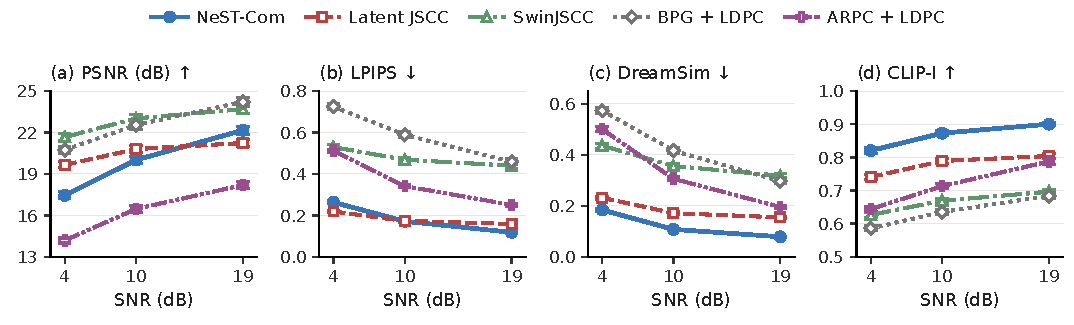
\includegraphics[width=\textwidth]{figure2.pdf}
\caption{Five-method performance on common500 at $N=1024$. Markers and error bars show source means and pointwise 95\% bootstrap intervals after averaging three channel realizations per image. Higher PSNR/CLIP-I and lower LPIPS-Alex/DreamSim are favorable.}
\label{fig:performance}
\end{figure*}

\subsection{Experimental Setup}
The main evaluation uses 500 ImageNet validation images~\cite{imagenet}, denoted common500, at $256\times256$ resolution, with $N=1024$ and SNRs of 4, 10, and 19~dB. All methods use the same total symbol budget and nominal $E_s=2$. A separate set of 1000 calibration images selects the offline policy by maximizing mean DINOv2 ViT-L/14 image-feature cosine similarity~\cite{dinov2}.

We compare NeST-Com with Latent JSCC, SwinJSCC~\cite{swinjscc}, BPG + LDPC, and ARPC + LDPC. Latent JSCC is our convolutional baseline mapping the tokenizer's continuous latent to channel symbols, trained with image MSE, LPIPS, and normalized-latent consistency losses. SwinJSCC is adapted to $256\times256$ inputs and the $N=1024$ frame, including its protected mask/power signaling. Both JSCC baselines use the same 20\,000 training images, and Latent JSCC shares $\Dc$ with NeST-Com. We use the 100k-update Latent JSCC and adapted 200k-update SwinJSCC checkpoints. BPG~\cite{bpg} selects resolution and quantization to fit the payload. ARPC uses its native scale presets and the authors' frozen weights; its caption is counted in the payload. Each implementation includes its required signaling in the symbol budget.

We measure pixel fidelity with PSNR, perceptual similarity with LPIPS-Alex~\cite{lpips} and DreamSim~\cite{dreamsim}, and image-feature similarity with CLIP-I, the image--image cosine of CLIP ViT-L/14 embeddings~\cite{clip}. DreamSim and CLIP use fixed $224\times224$ preprocessing and FP32 inference. We first average each source's three channel realizations, including fixed gray outputs from rejected digital receptions. Error bars are pointwise 95\% source-bootstrap confidence intervals (CIs); differences use source-paired intervals. Pairing is by source image, since methods retain their original noise namespaces. A matched 100-image subset supports the larger-budget and ARPC sensitivity experiments.

\subsection{Comparison With Existing Methods}
Fig.~\ref{fig:performance} shows that NeST-Com attains the lowest DreamSim and highest CLIP-I means at all three tested SNRs. At 10~dB, its DreamSim is 0.108, compared with 0.171 for Latent JSCC and 0.306 for ARPC; the corresponding CLIP-I values are 0.873, 0.789, and 0.713. Its PSNR exceeds ARPC by 3.26--3.97~dB across the three points. SwinJSCC and BPG achieve higher PSNR than NeST-Com throughout. Latent JSCC also has higher PSNR at 4 and 10~dB: 19.66 versus 17.45~dB and 20.80 versus 20.01~dB. For LPIPS, Latent JSCC leads at 4~dB, the methods are close at 10~dB (0.1733 versus 0.1715; paired CI includes zero), and NeST-Com leads at 19~dB. On the matched 100-image subset, replacing ARPC's original sampling ($\tau=0.5$) with argmax or $\tau=0.25$ changes mean PSNR by at most approximately 0.15~dB, while both alternatives worsen LPIPS and DreamSim at 4~dB. These tested choices do not account for the multi-dB PSNR gap.

Fig.~\ref{fig:qualitative} shows two previously selected development examples at 10~dB. NeST-Com and Latent JSCC preserve the pastry arrangement and the dog's silhouette, with clearer pastry folds and facial fur in the NeST-Com examples. SwinJSCC smooths detail, BPG introduces visible blocks, and ARPC produces texture with changes in shape and appearance. For the dog, Latent JSCC has lower LPIPS (0.203 versus 0.233), whereas NeST-Com has lower DreamSim (0.114 versus 0.166).

\begin{figure*}[t]
\centering
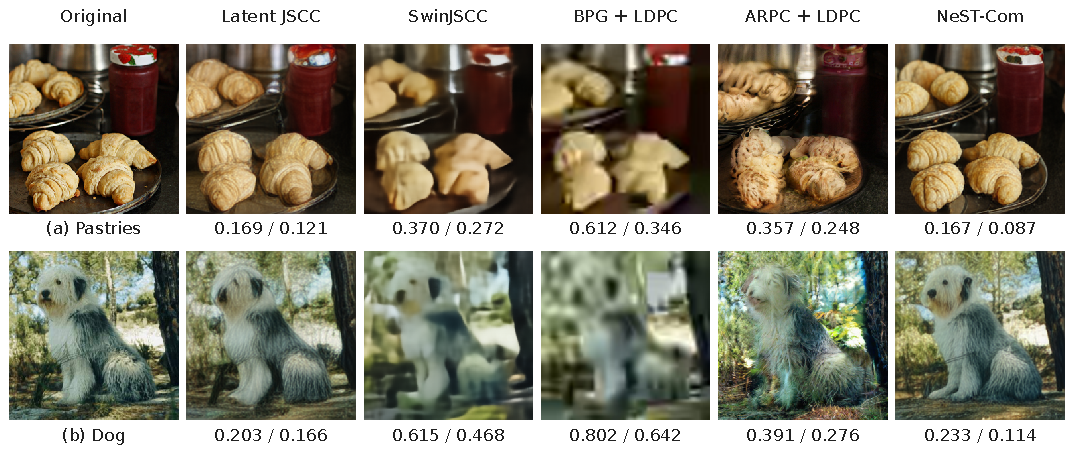
\includegraphics[width=\textwidth]{figure3.pdf}
\caption{Qualitative reconstructions at $N=1024$ and 10~dB for two selected development examples: (a) pastries and (b) a dog. Values below each reconstruction denote LPIPS-Alex$\downarrow$ / DreamSim$\downarrow$ for the displayed realization.}
\label{fig:qualitative}
\end{figure*}

\subsection{Effect of Within-Scale Endpoints}
We compare WHOLE, which permits complete-scale endpoints, with PARTIAL, which additionally permits the quarter-scale endpoints in~\eqref{eq:endpoints}. The tokenizer, prior, entropy coder, and image decoder are shared. The two endpoint sets are calibrated separately and select the same MCS at each tested SNR. Table~\ref{tab:endpoints} reports PARTIAL minus WHOLE on common500.

At 10~dB, finer endpoints raise utilization from 77.70\% to 95.21\%, improve PSNR by 0.701~dB, and reduce DreamSim by 0.0240. Across all three SNRs, PSNR improves by 0.32--0.70~dB with positive CIs, and DreamSim decreases with negative CIs. With shared model components and matched MCS, this comparison supports the benefit of endpoint granularity together with calibrated actual-length fitting: additional boundary tokens can be retained when the next complete scale would overflow the frame.
\begin{table}[t]
\centering
\caption{Within-scale endpoint gains on common500}
\label{tab:endpoints}
\begingroup
\footnotesize
\setlength{\tabcolsep}{3pt}
\renewcommand{\arraystretch}{1.15}
\begin{tabular}{@{}rccc@{}}
\toprule
SNR & $\eta$ (\%), W/P & $\Delta$PSNR (dB) & $\Delta$DreamSim \\
\midrule
4 dB & 73.81/93.08 & \CI{+0.616}{0.564}{0.673} & \CI{-0.0207}{-0.0233}{-0.0183} \\[3pt]
10 dB & 77.70/95.21 & \CI{+0.701}{0.637}{0.766} & \CI{-0.0240}{-0.0270}{-0.0212} \\[3pt]
19 dB & 85.24/94.73 & \CI{+0.319}{0.290}{0.349} & \CI{-0.0030}{-0.0037}{-0.0024} \\
\bottomrule
\end{tabular}
\endgroup
\par\smallskip
\begin{minipage}{\columnwidth}\footnotesize
W/P: WHOLE/PARTIAL. $\eta$ uses the terminated entropy length and source capacity in~\eqref{eq:budget}. Differences are PARTIAL minus WHOLE; brackets give source-paired 95\% CIs.
\end{minipage}
\end{table}


\subsection{Performance With a Larger Symbol Budget}
The $N=2048$ experiment examines whether ARPC's gap is explained by its full representation not fitting at $N=1024$. Each image uses two 1024-symbol subframes with their own protected headers. Table~\ref{tab:larger} compares adaptive configurations at 4 and 10~dB and complete-representation transmission at 19~dB, using 100 images and three channel realizations per image. All 300 receptions per method succeed in each reported condition.

When both complete representations are delivered at 19~dB, NeST-Com retains a 1.806~dB PSNR advantage and lower DreamSim. ARPC has lower DISTS~\cite{dists}: NeST-Com minus ARPC is $+0.0054$, with 95\% CI $[+0.0024,+0.0086]$. Representation and decoding also affect quality, with different perceptual criteria favoring different reconstructions. The full-system comparison includes these effects alongside the within-family endpoint gains in Table~\ref{tab:endpoints}.
\begin{table}[t]
\centering
\caption{NeST-Com minus ARPC at $N=2048$}
\label{tab:larger}
\begingroup
\footnotesize
\setlength{\tabcolsep}{3pt}
\renewcommand{\arraystretch}{1.15}
\begin{tabular}{@{}lcc@{}}
\toprule
Condition & $\Delta$PSNR (dB) & $\Delta$DreamSim \\
\midrule
4 dB, adaptive & \CI{+3.779}{3.493}{4.082} & \CI{-0.2658}{-0.2933}{-0.2386} \\[3pt]
10 dB, adaptive & \CI{+3.877}{3.688}{4.079} & \CI{-0.1174}{-0.1309}{-0.1049} \\[3pt]
19 dB, full & \CI{+1.806}{1.742}{1.871} & \CI{-0.0086}{-0.0119}{-0.0052} \\
\bottomrule
\end{tabular}
\endgroup
\par\smallskip
\begin{minipage}{\columnwidth}\footnotesize
Source-paired 95\% CIs over 100 images, each with three noise realizations. Full denotes delivery of both methods\textquotesingle{} complete representations.
\end{minipage}
\end{table}


\subsection{Computational Cost}
Table~\ref{tab:latency} reports software processing latency at 10~dB on an RTX PRO 6000 Blackwell GPU with six assigned CPU cores. Measurements use batch size one, 16 development images, three warmups per method/SNR setting, and three measured repetitions per image. TX and RX include source handling, channel-code processing, and reconstruction; total is TX plus RX. Model initialization, channel-noise generation, and radio transmission time are excluded. BPG's TX includes adaptive resolution/quantization search. Shared-machine load was recorded during measurement.

NeST-Com takes 619.71~ms per image, compared with 42--45~ms for continuous JSCC, 1520.30~ms for ARPC, and 2293.01~ms for adaptive BPG. Its 398.82~ms receiver cost includes local probability reconstruction and next-scale completion. These measurements expose the processing cost accompanying its perceptual and image-feature similarity gains.
\begin{table}[t]
\centering
\caption{Mean software processing latency at $N=1024$, 10~dB (ms/image)}
\label{tab:latency}
\begingroup
\footnotesize
\setlength{\tabcolsep}{3pt}
\renewcommand{\arraystretch}{1.15}
\begin{tabular}{@{}lrrr@{}}
\toprule
Method & TX & RX & Total \\
\midrule
NeST-Com & 220.89 & 398.82 & 619.71 \\[3pt]
Latent JSCC & 17.97 & 24.51 & 42.48 \\[3pt]
SwinJSCC & 24.81 & 19.89 & 44.69 \\[3pt]
BPG + LDPC & 2269.87 & 23.15 & 2293.01 \\[3pt]
ARPC + LDPC & 719.12 & 801.18 & 1520.30 \\
\bottomrule
\end{tabular}
\endgroup
\par\smallskip
\begin{minipage}{\columnwidth}\footnotesize
RTX PRO 6000 Blackwell, six CPU cores, batch size one. Total is TX + RX; model initialization, channel-noise generation, and radio transmission time are excluded.
\end{minipage}
\end{table}

